\documentclass[12pt,a4paper]{article}

\usepackage[utf8]{inputenc}
\usepackage[english]{babel}
\usepackage{amssymb, amsmath}
\usepackage{fullpage}
\usepackage{parskip}
\usepackage{url}
\usepackage[dvipsnames]{xcolor}
\usepackage{enumitem}
\usepackage{graphicx}

\renewcommand{\vec}[1]{\mathbf{#1}}
\newcommand{\from}{\colon}
\newcommand{\IR}{\mathbb{R}}
\newcommand{\IN}{\mathbb{N}}
\newcommand{\norm}[1]{\left\|#1\right\|}

\pagestyle{empty}

\begin{document}
    
    %%%%%%%%%%%%%%%%%%%%%%%%%%%%%%%%%%%%%%%%%%%%%%%%%%
    Differential equations: phase portraits
    \hfill
    ELTE, autumn 2019/20
    \\
    \hspace*{\fill} {\tiny R.A., \today}
    %%%%%%%%%%%%%%%%%%%%%%%%%%%%%%%%%%%%%%%%%%%%%%%%%%
    
    %%%%%%%%%%%%%%%%%%%%%%%%%%%%%%%%%%%%%%%%%%%%%%%%%%
    \setcounter{section}{3}
    %%%%%%%%%%%%%%%%%%%%%%%%%%%%%%%%%%%%%%%%%%%%%%%%%%
    
    %%%%%%%%%%%%%%%%%%%%%%%%%%%%%%%%%%%%%%%%%%%%%%%%%%
    \subsection{}
    %%%%%%%%%%%%%%%%%%%%%%%%%%%%%%%%%%%%%%%%%%%%%%%%%%
    
    Fix $m > 0$ and $g > 0$.
    %
    Consider 
    $
        E_\text{I}(x, v) := \tfrac12 m v^2 + g x
    $
    for
    $(x, v) \in \IR^2$.
    %
    \begin{itemize}
    \item 
        In the $x$-$v$ plane,
        sketch the level curves of $E_\text{I}$.
    \item
        If $E_\text{I}(x(t), v(t))$ is constant
        and $\dot{x} = v$, what is $\dot{v}$?
    \item
        Sketch $x$ and $v$ as functions of $t$.
    \item
        Compute $F = m \ddot{x}$.
    \end{itemize}

    %%%%%%%%%%%%%%%%%%%%%%%%%%%%%%%%%%%%%%%%%%%%%%%%%%
    \subsection{}
    %%%%%%%%%%%%%%%%%%%%%%%%%%%%%%%%%%%%%%%%%%%%%%%%%%
    
    Same for $E_\text{II}(x, v) := \tfrac12 m v^2 + \tfrac12 k x^2$,
    where $k > 0$.
    
    %%%%%%%%%%%%%%%%%%%%%%%%%%%%%%%%%%%%%%%%%%%%%%%%%%
    \subsection{}
    %%%%%%%%%%%%%%%%%%%%%%%%%%%%%%%%%%%%%%%%%%%%%%%%%%
    
    Suppose $F = m \ddot{x} \stackrel{!}{=} - k x - \gamma v$, where $k > 0$ and $\gamma > 0$.
    %
    Sketch the orbits in phase space.
    
    
    %%%%%%%%%%%%%%%%%%%%%%%%%%%%%%%%%%%%%%%%%%%%%%%%%%
    \subsection{}
    %%%%%%%%%%%%%%%%%%%%%%%%%%%%%%%%%%%%%%%%%%%%%%%%%%
    
    Given the vectorfield $x \mapsto A \, x$ in $\IR^2$,
    suggest a plausible matrix $A$.
    
    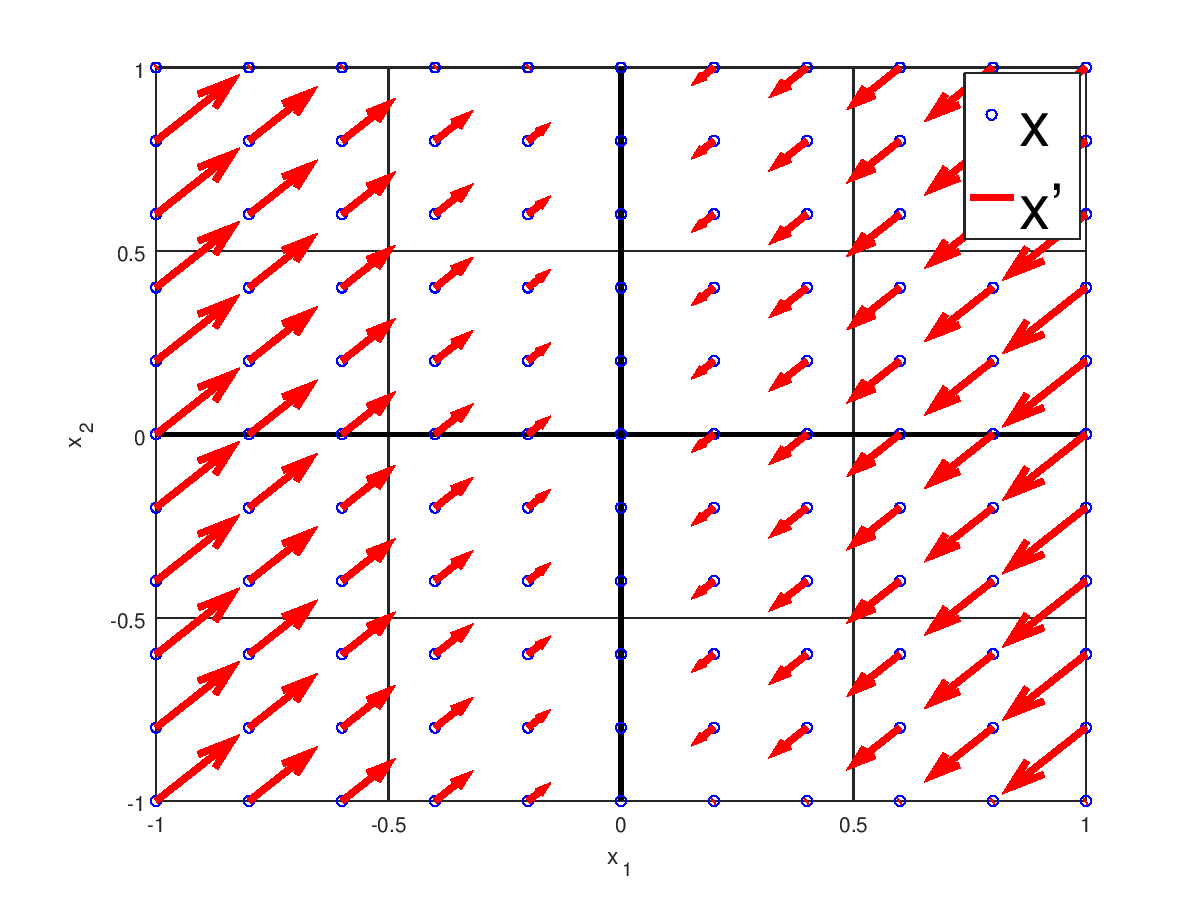
\includegraphics[width=0.25\textwidth]{A/2.png}
    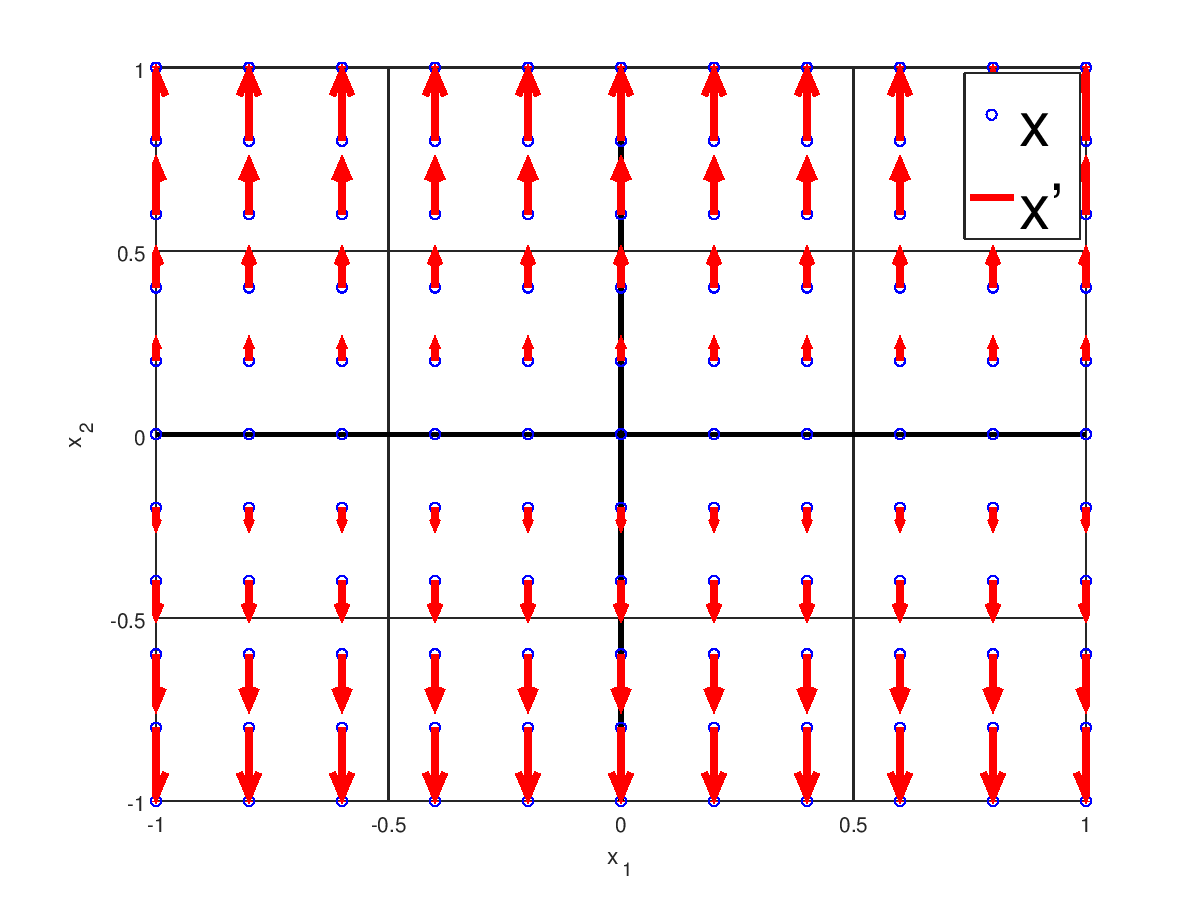
\includegraphics[width=0.25\textwidth]{A/3.png}
    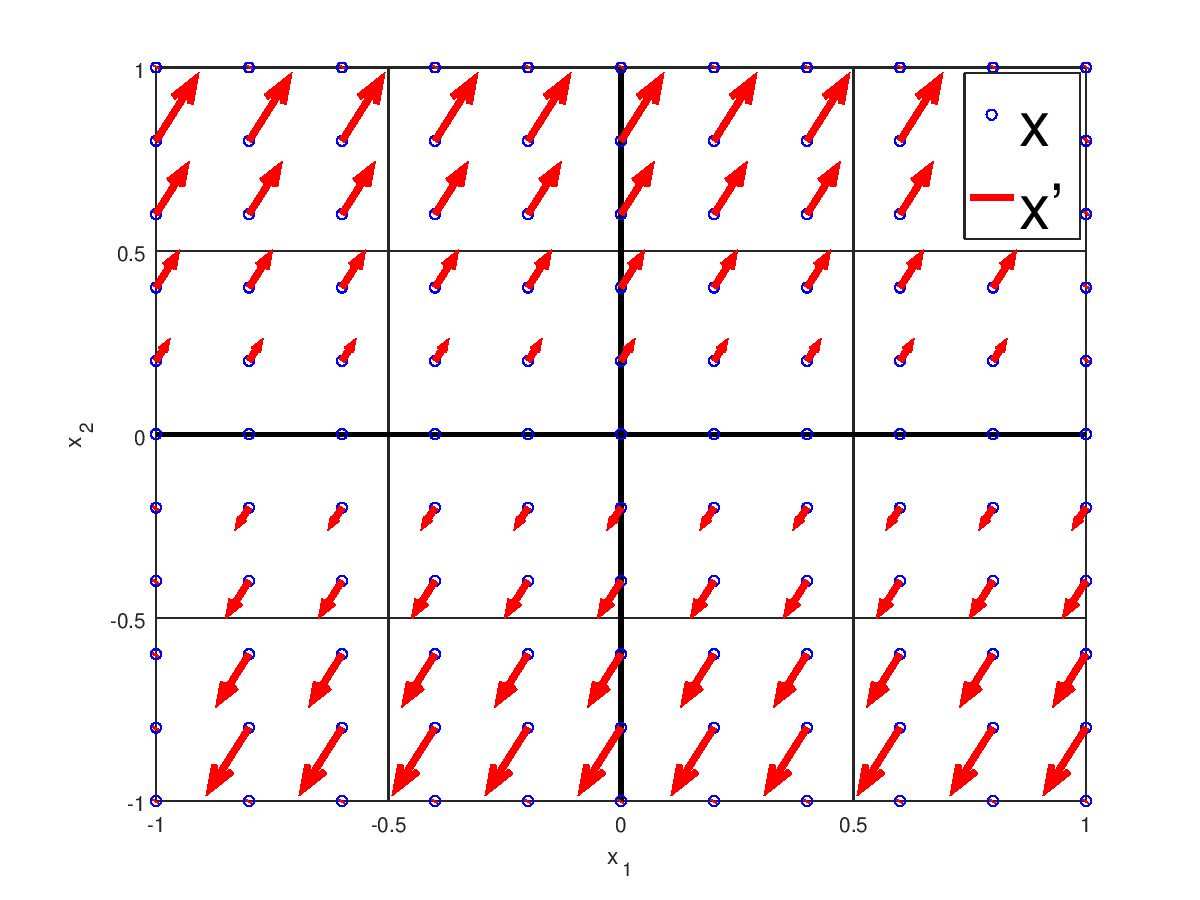
\includegraphics[width=0.25\textwidth]{A/6.png}
    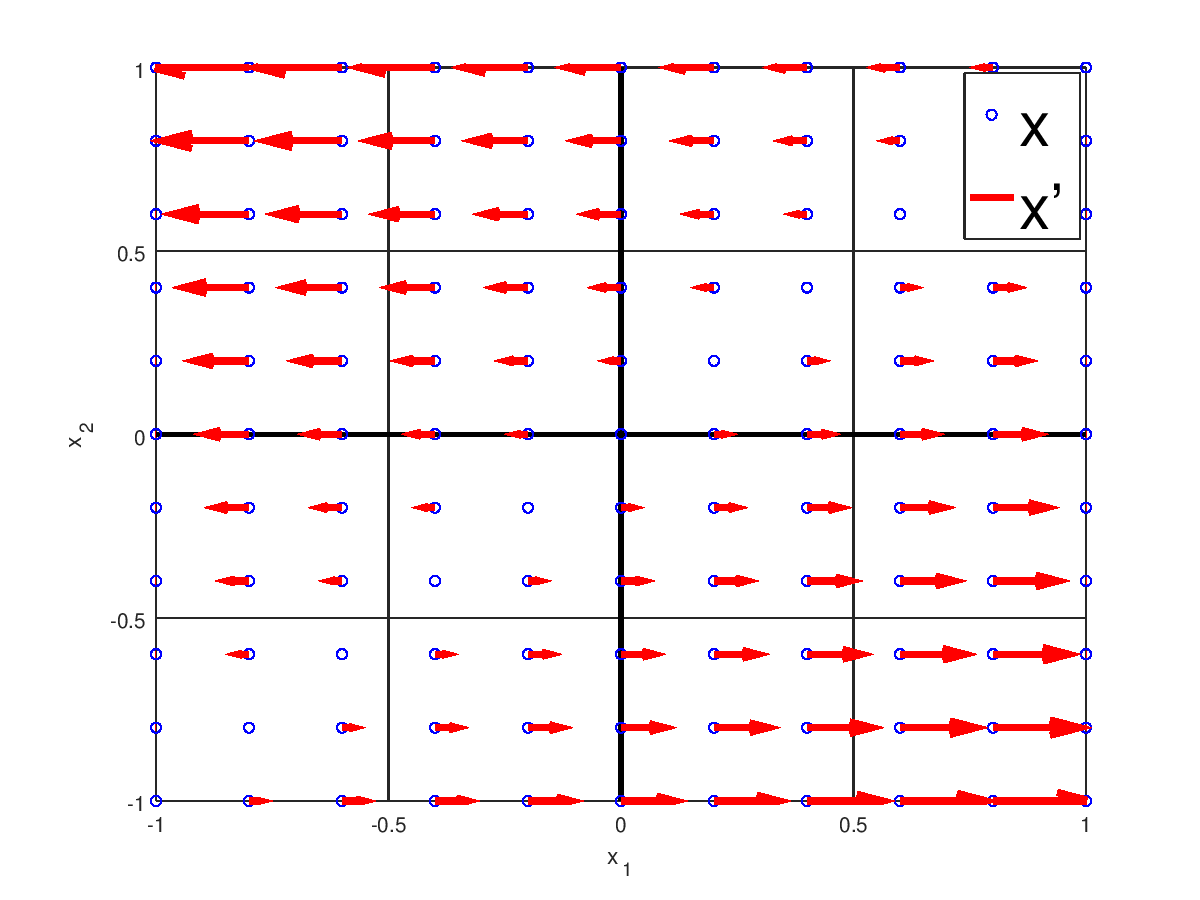
\includegraphics[width=0.25\textwidth]{A/15.png}
    %
    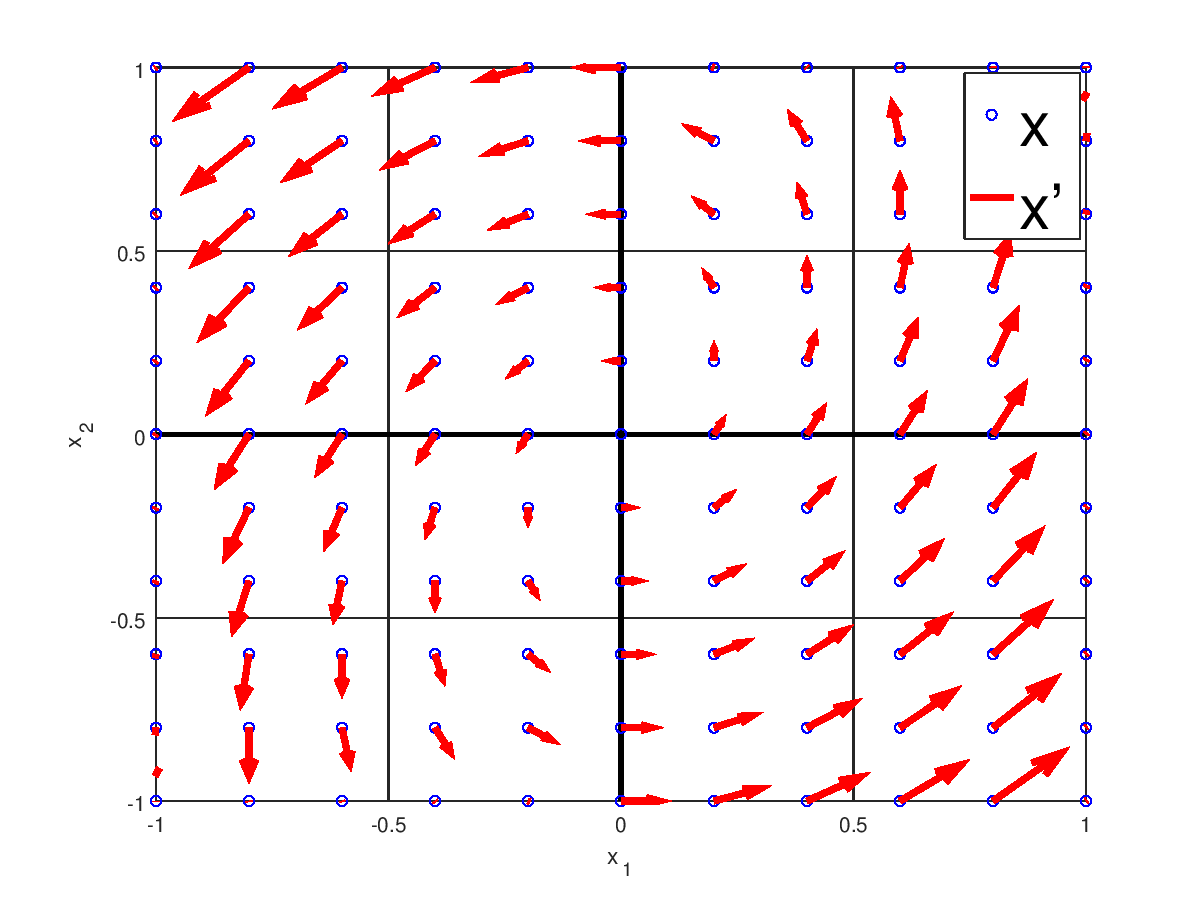
\includegraphics[width=0.25\textwidth]{A/8.png}
    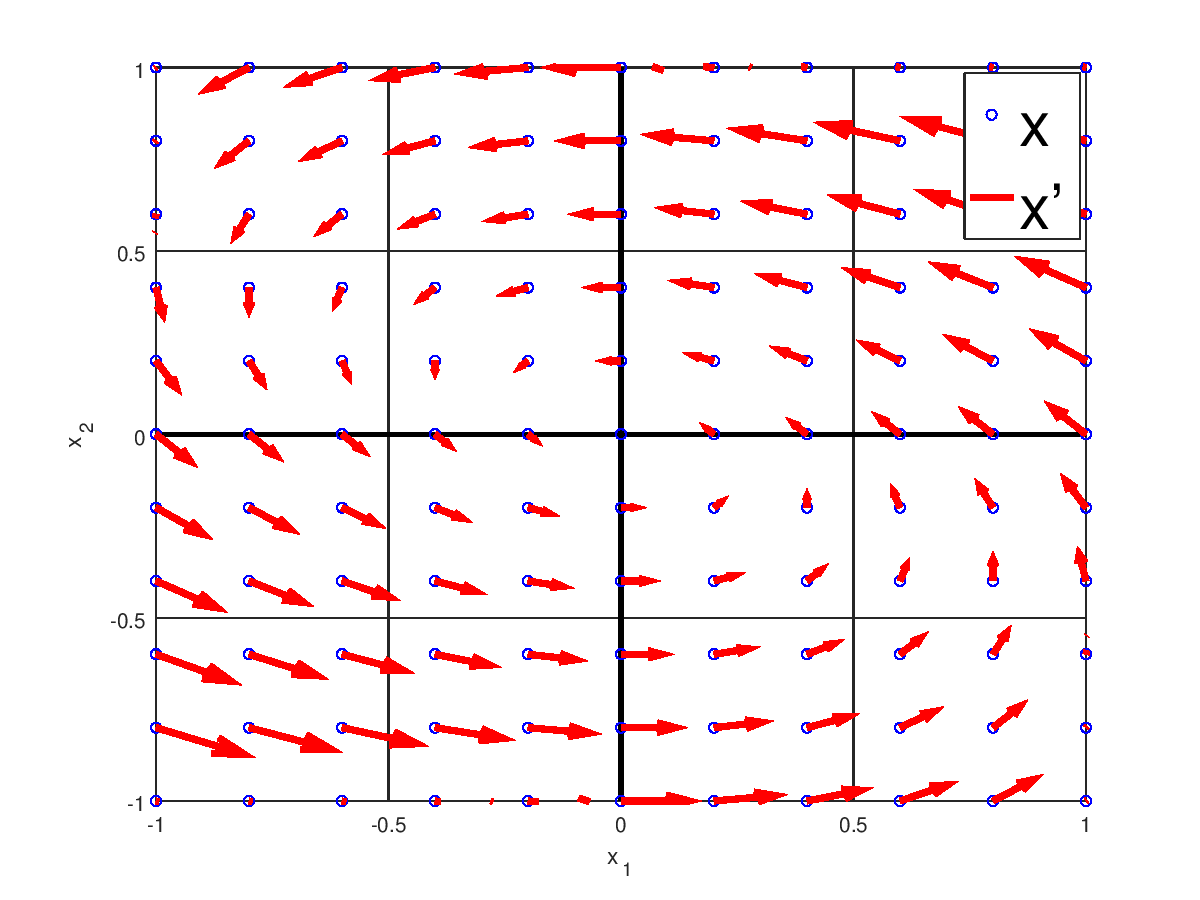
\includegraphics[width=0.25\textwidth]{A/11.png}
    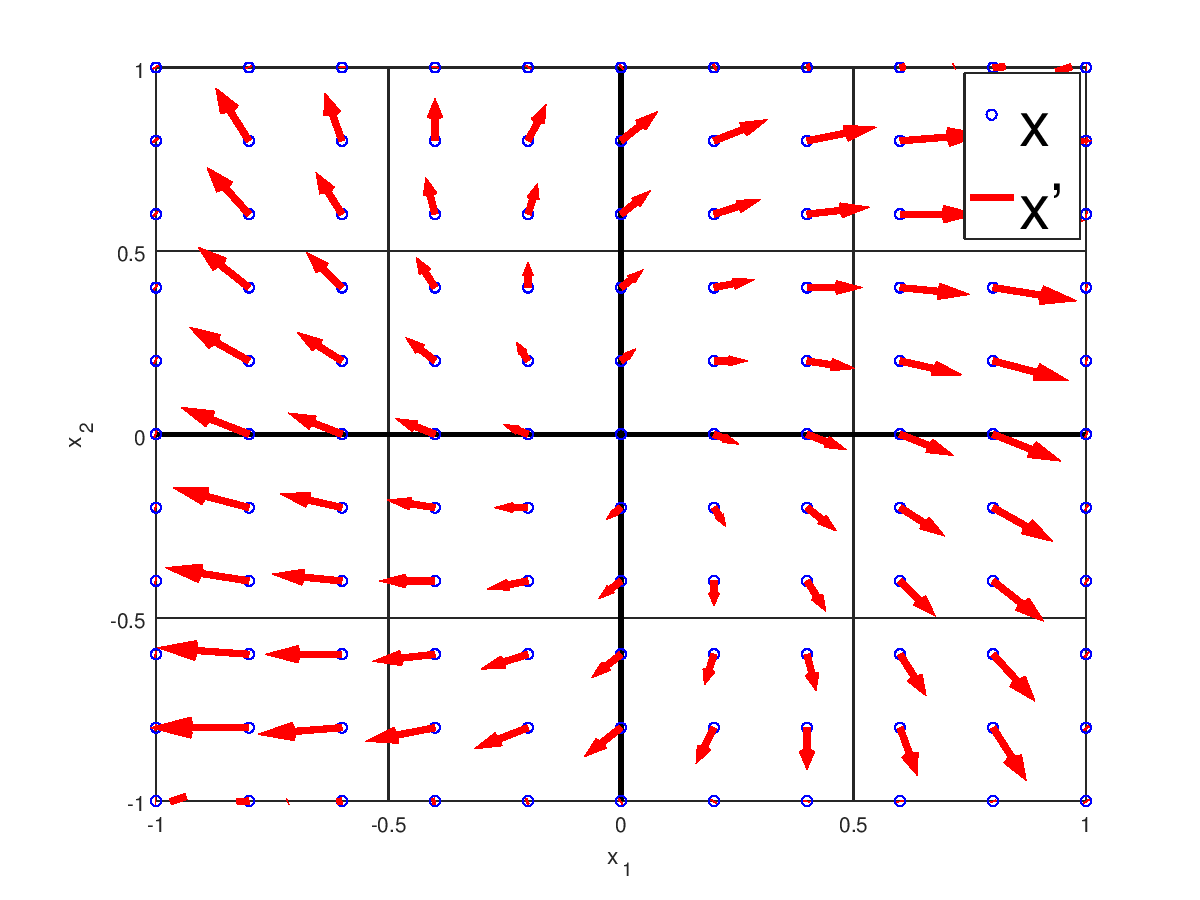
\includegraphics[width=0.25\textwidth]{A/12.png}
    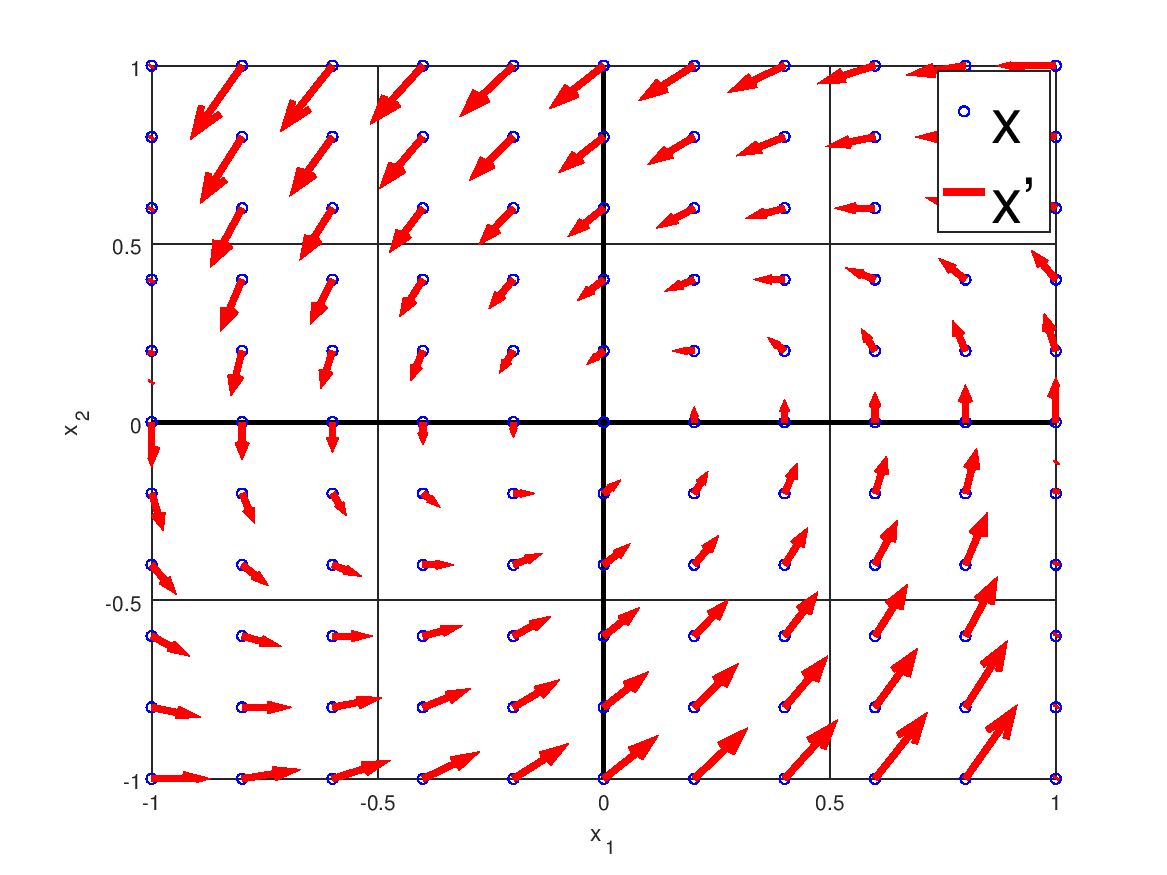
\includegraphics[width=0.25\textwidth]{A/19.png}
    %
    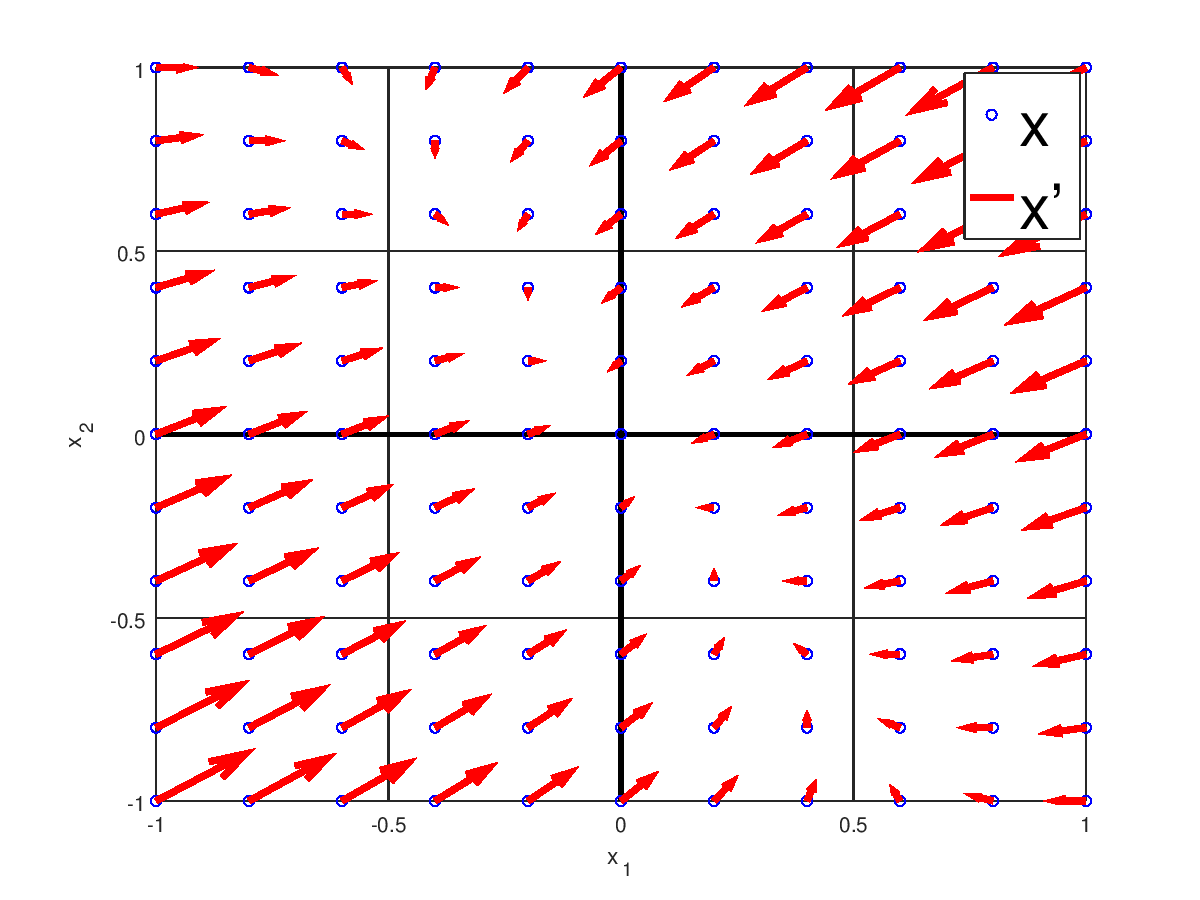
\includegraphics[width=0.25\textwidth]{A/1.png}
    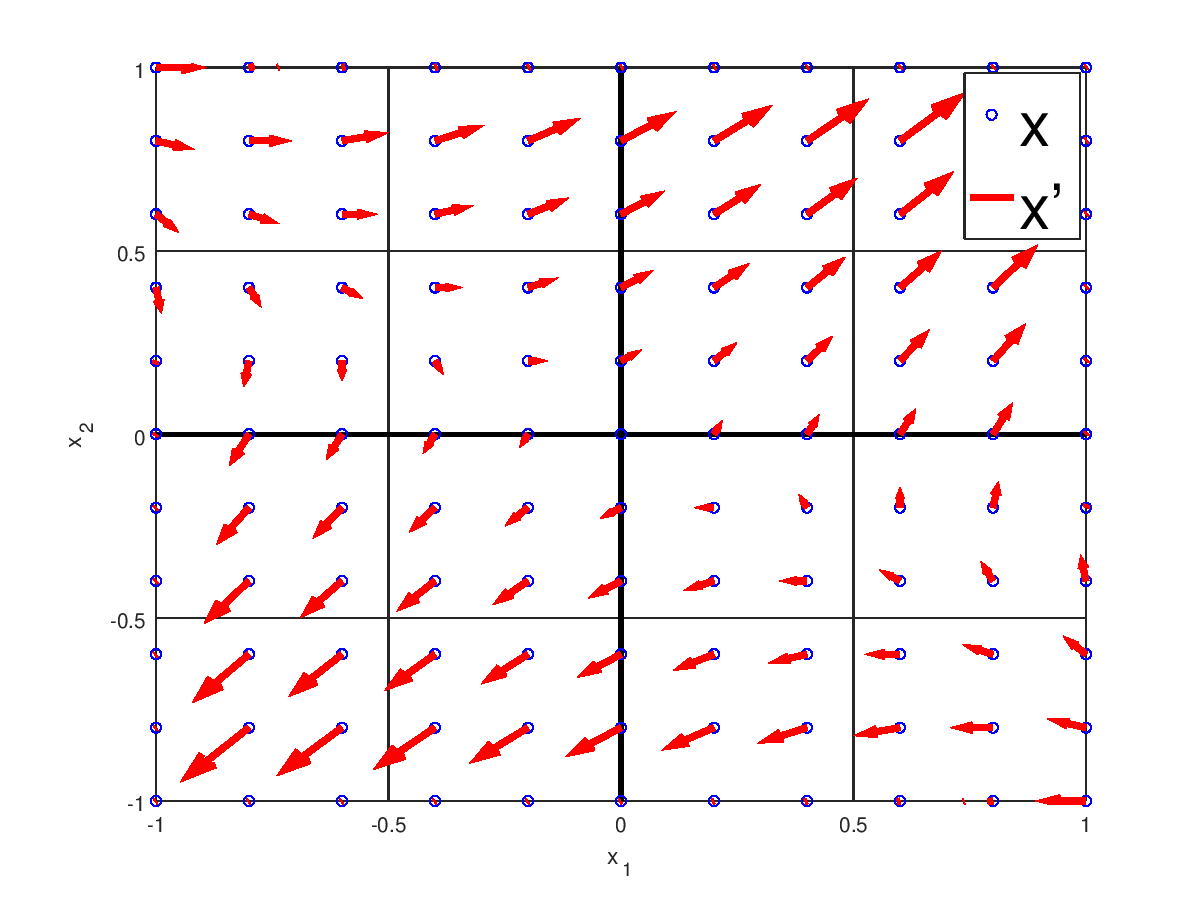
\includegraphics[width=0.25\textwidth]{A/5.png}
    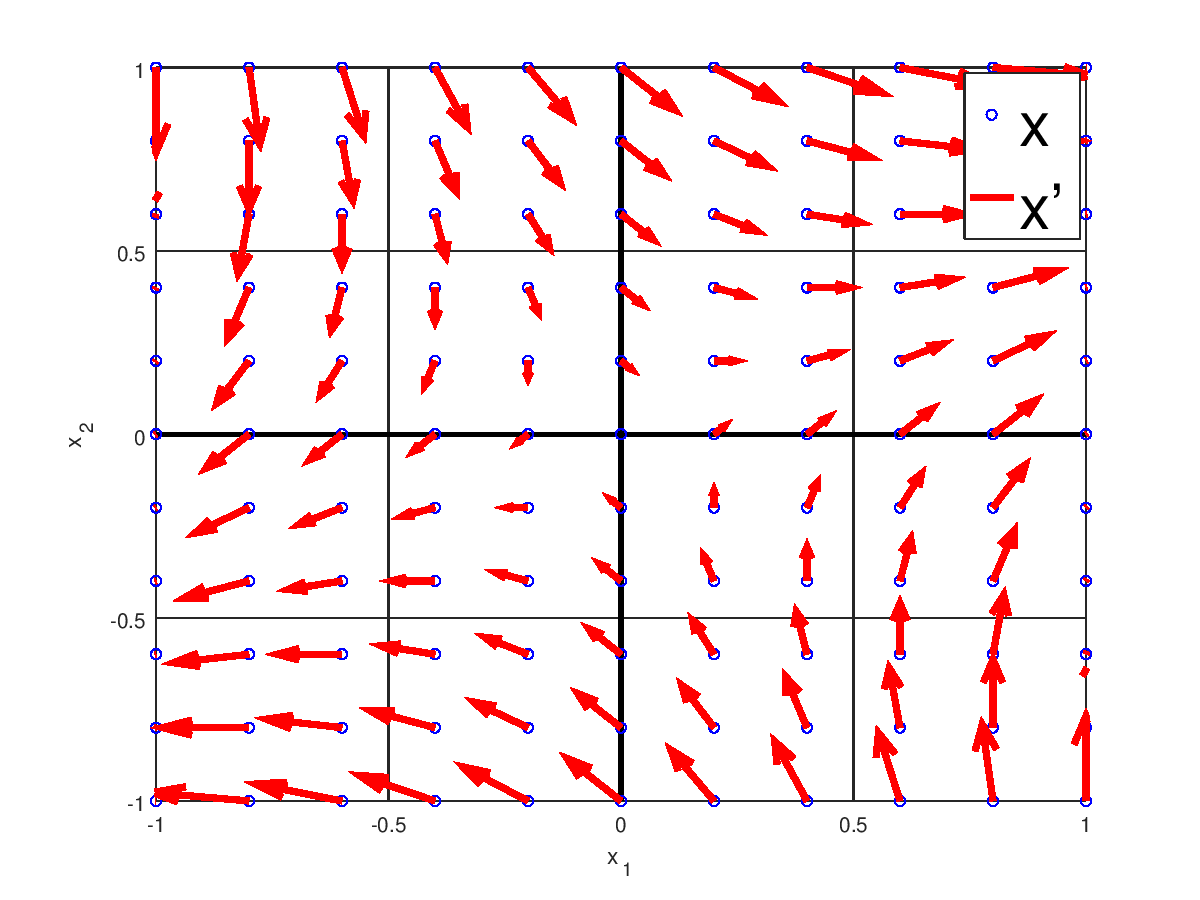
\includegraphics[width=0.25\textwidth]{A/10.png}
    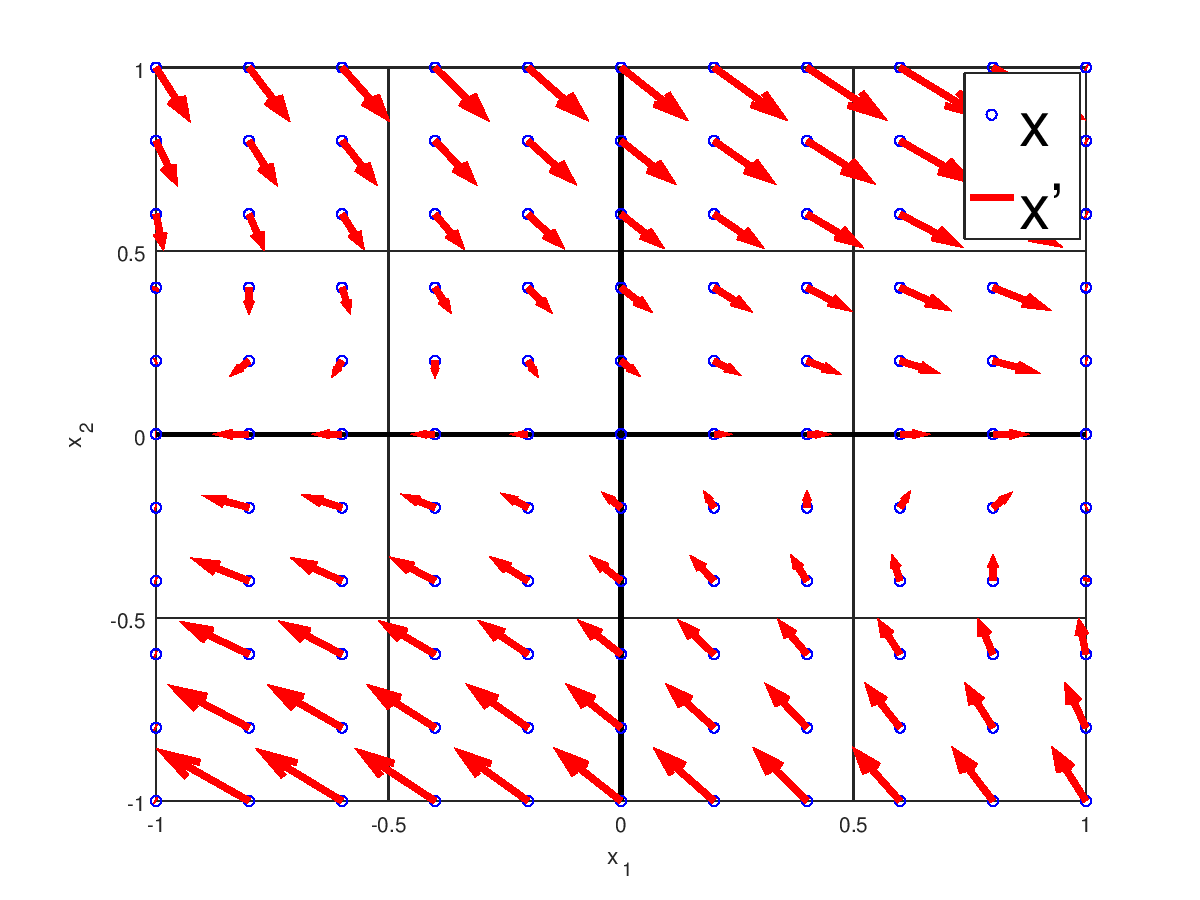
\includegraphics[width=0.25\textwidth]{A/18.png}
    
%     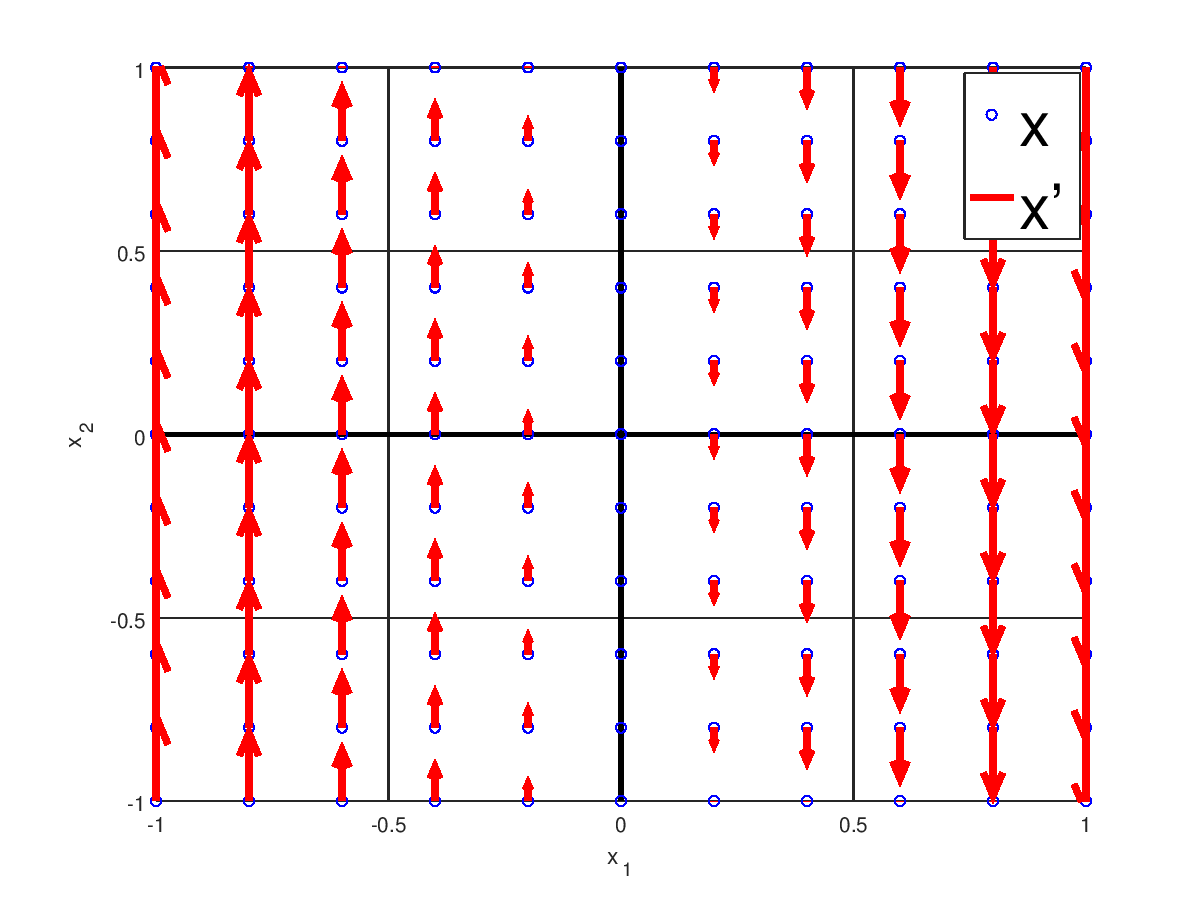
\includegraphics[width=0.25\textwidth]{A/13.png}
%     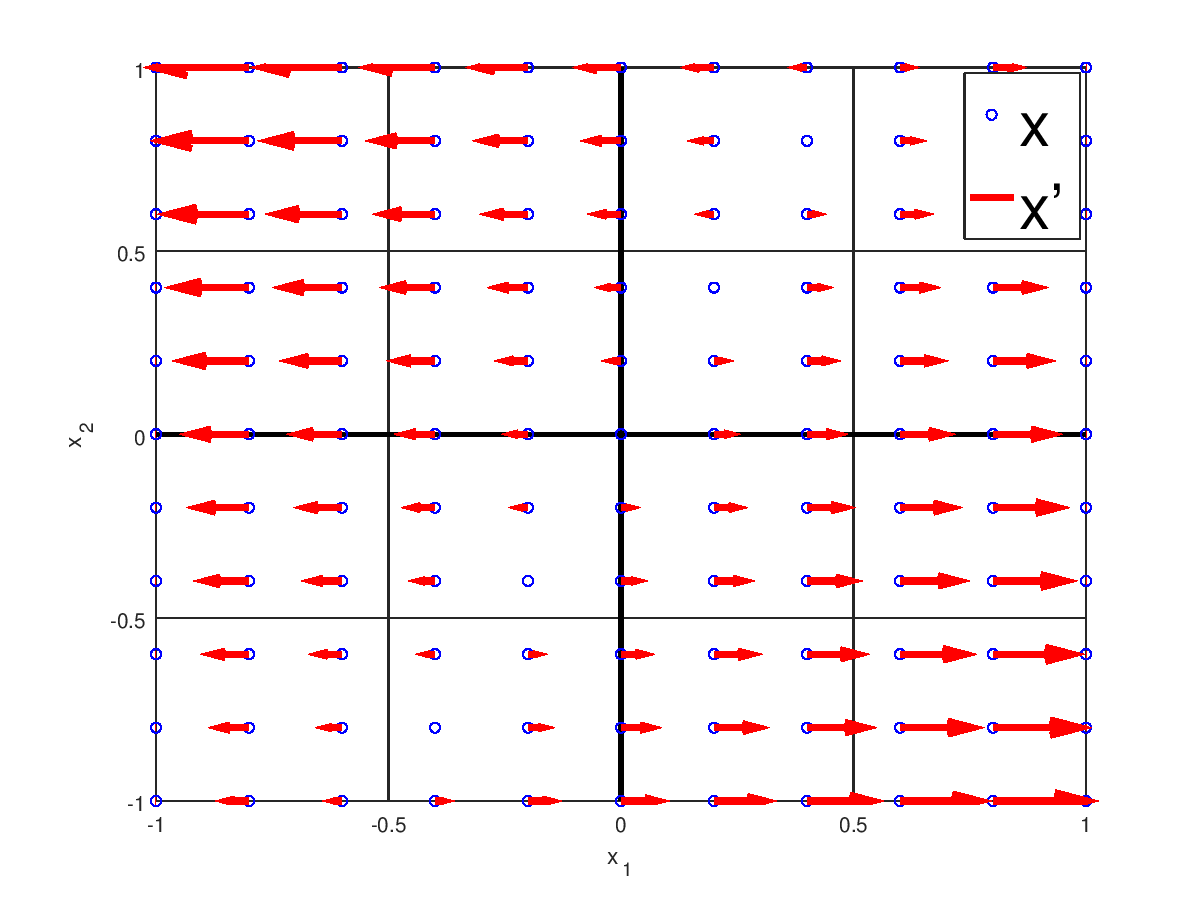
\includegraphics[width=0.25\textwidth]{A/14.png}
%     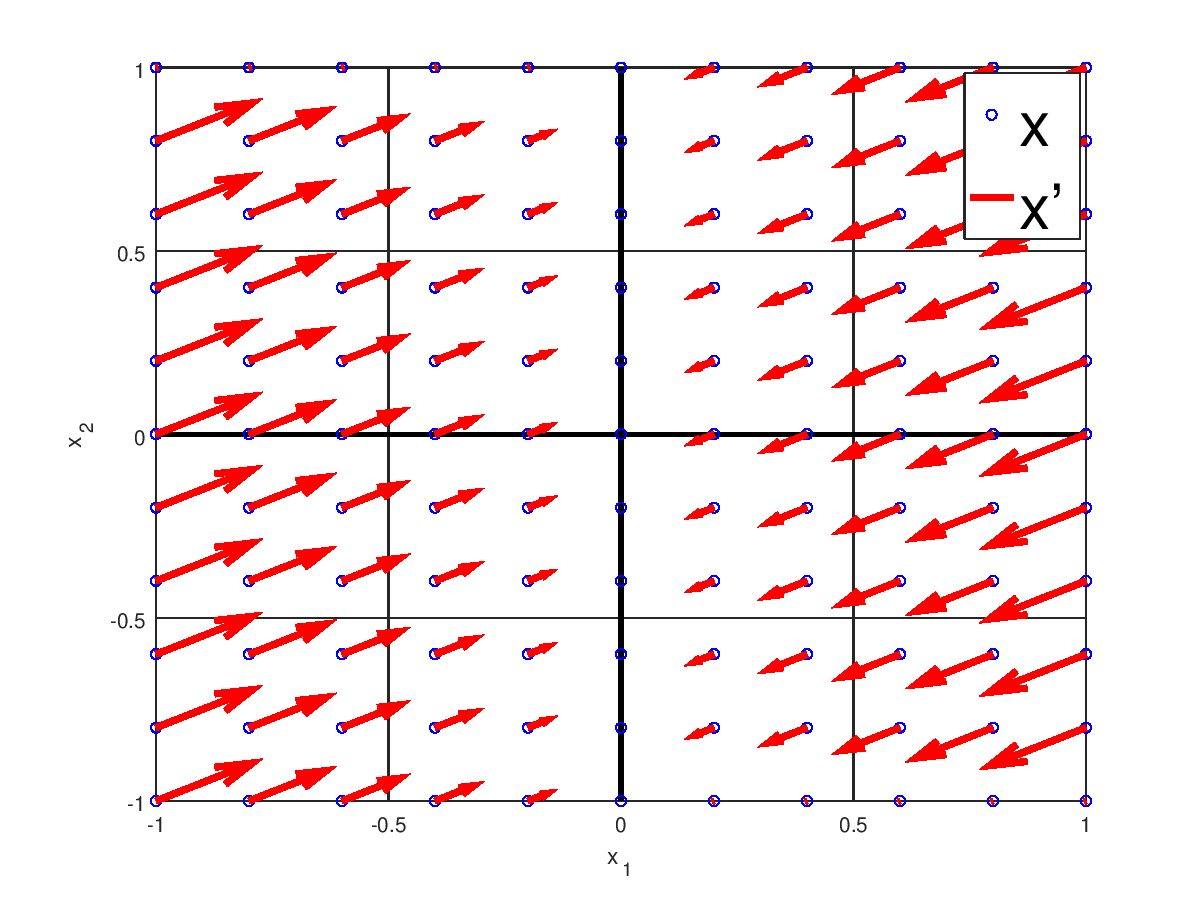
\includegraphics[width=0.25\textwidth]{A/16.png}
%     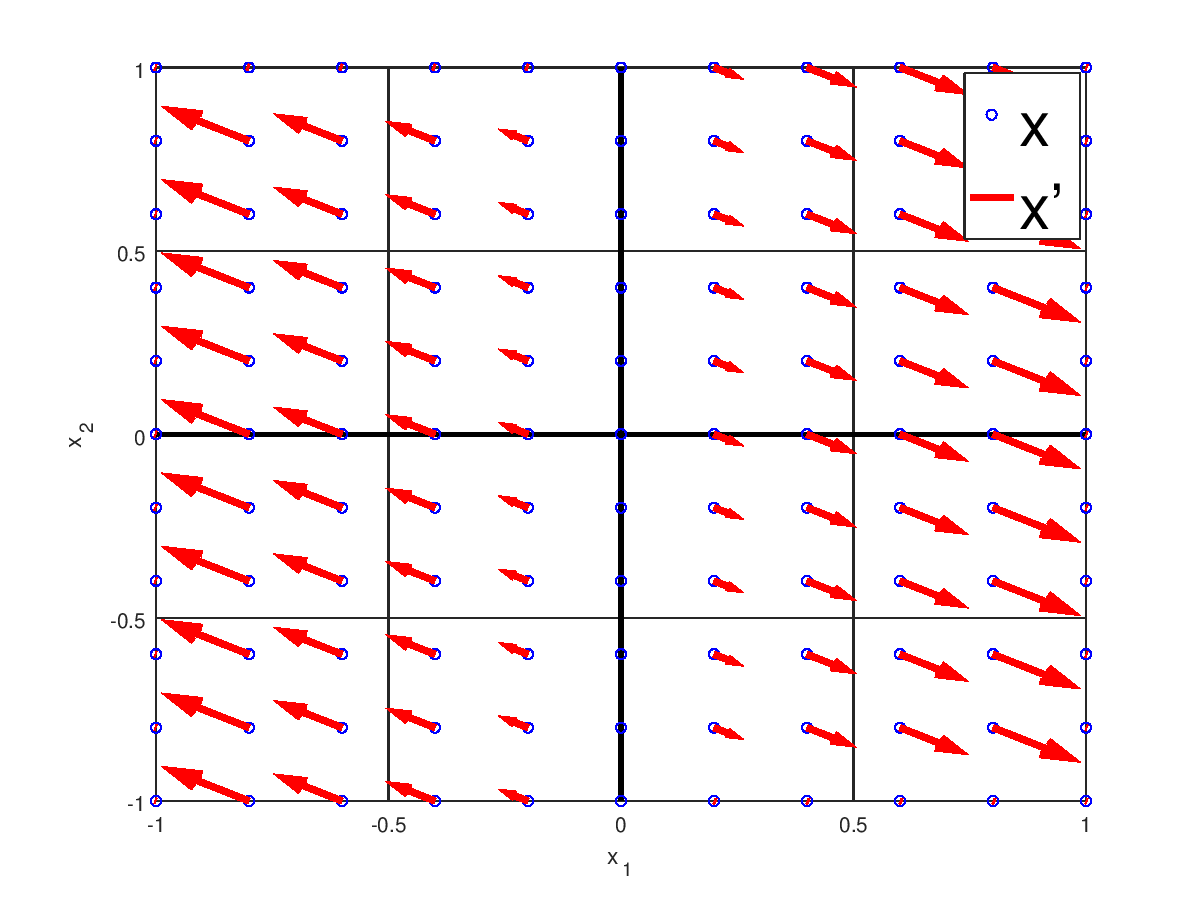
\includegraphics[width=0.25\textwidth]{A/7.png}
%     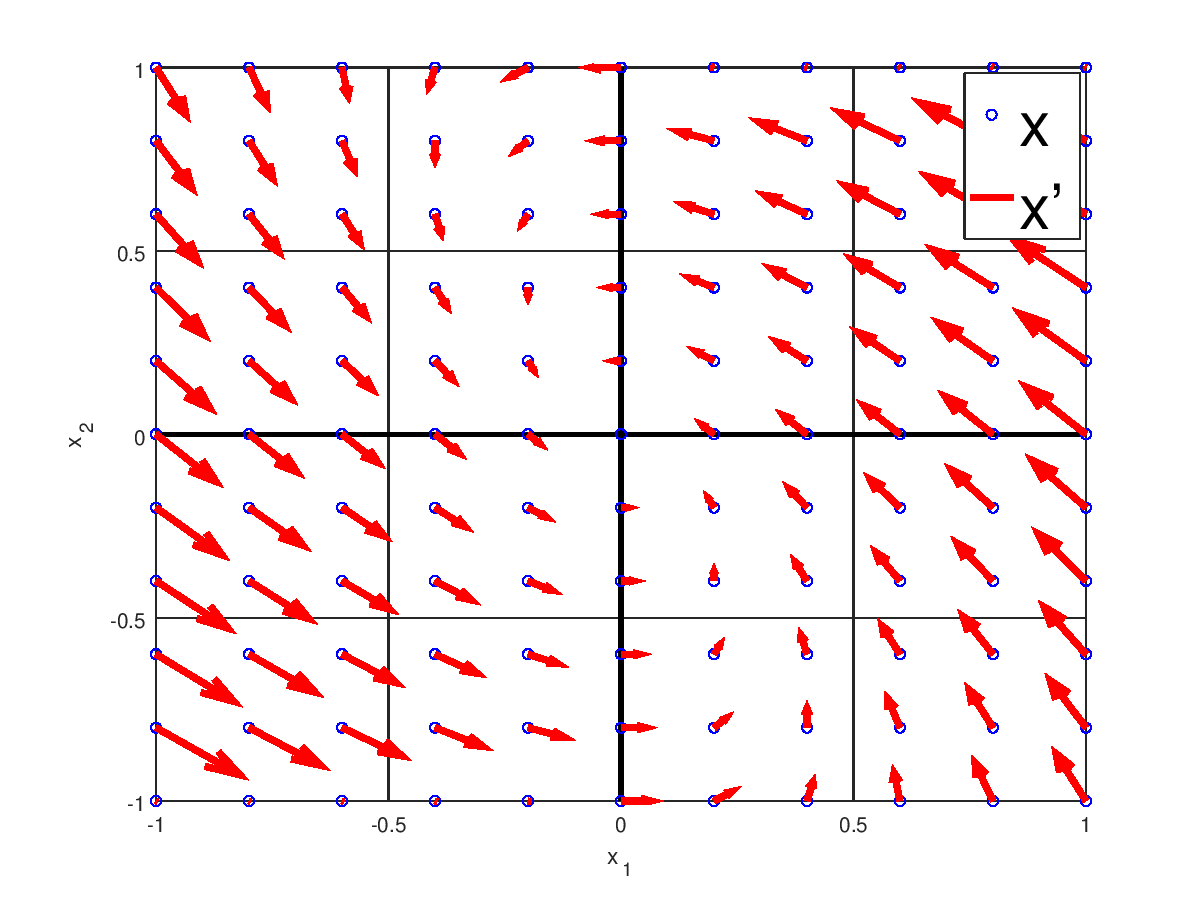
\includegraphics[width=0.25\textwidth]{A/17.png}
%     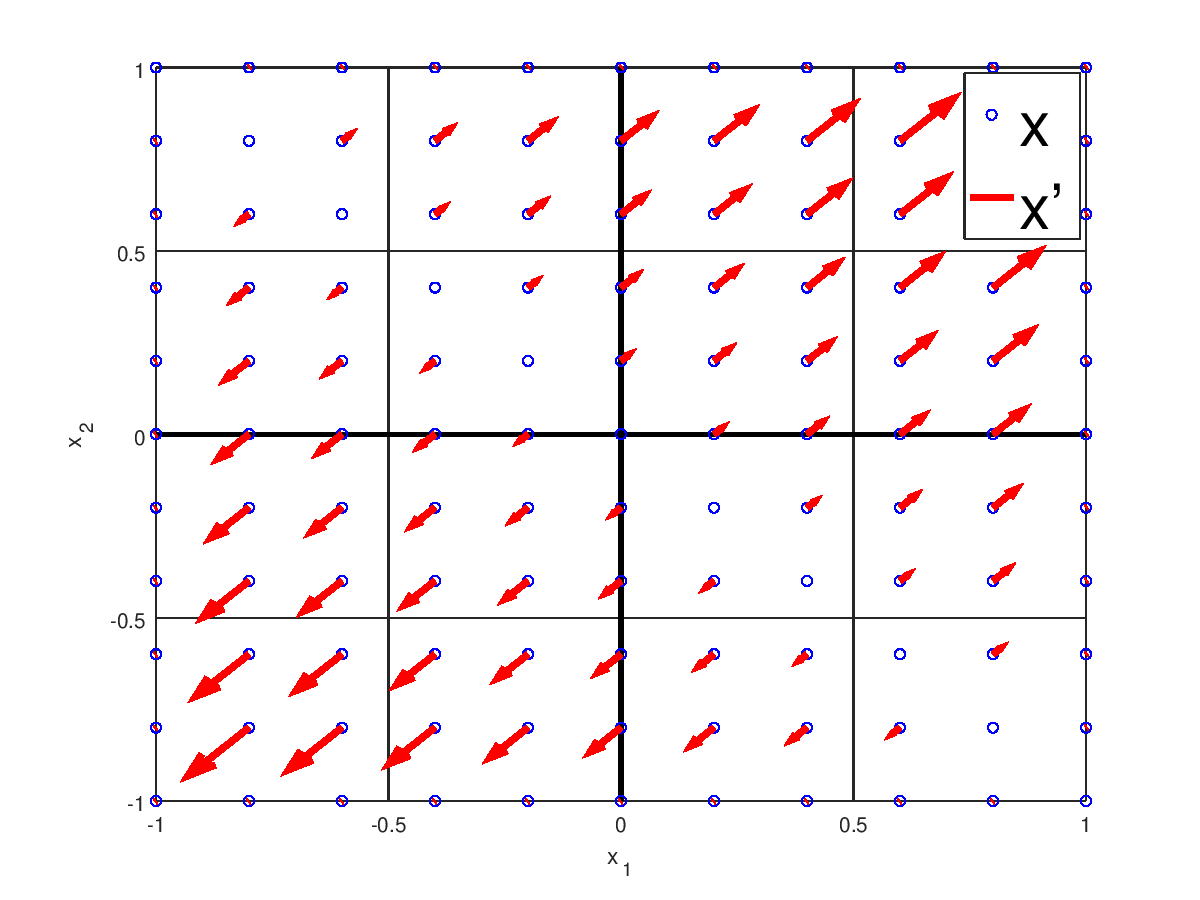
\includegraphics[width=0.25\textwidth]{A/4.png}
%     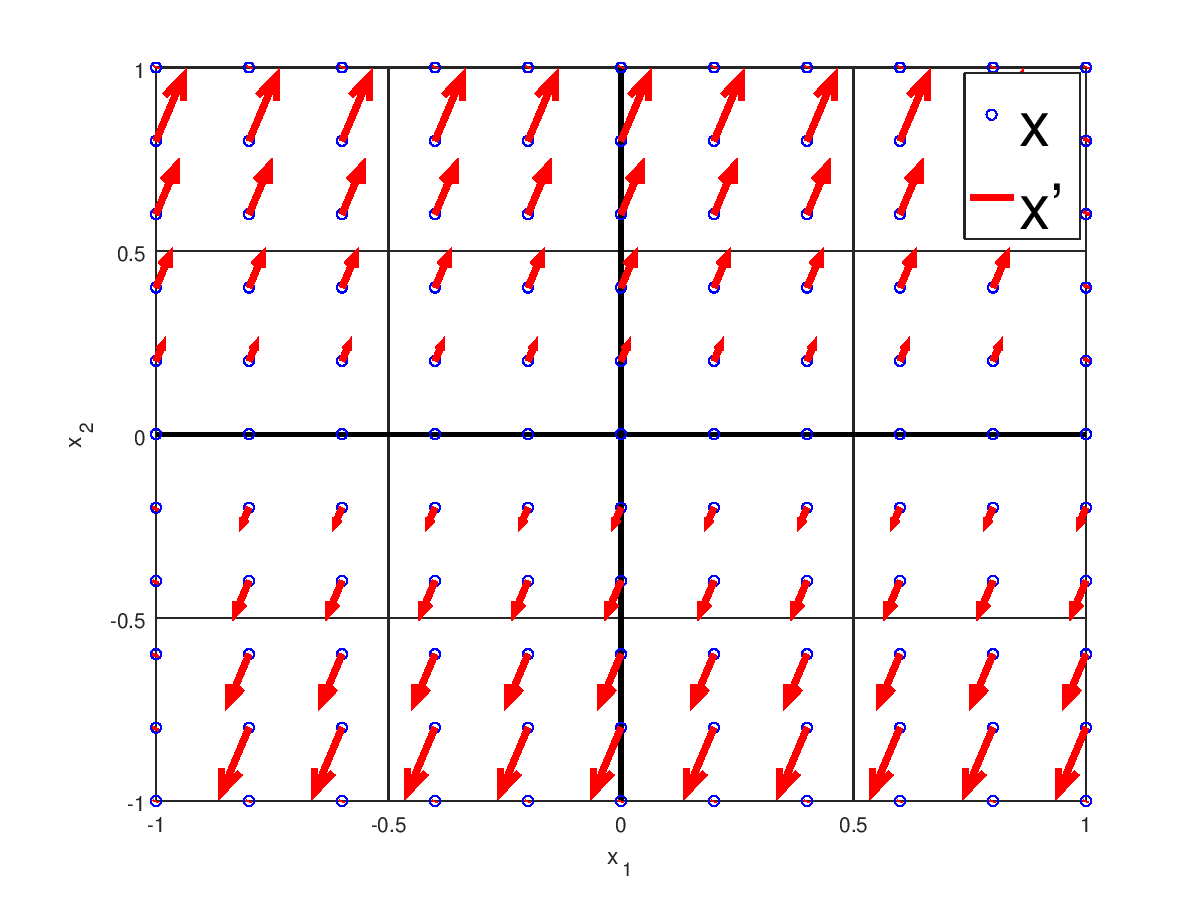
\includegraphics[width=0.25\textwidth]{A/9.png}
%     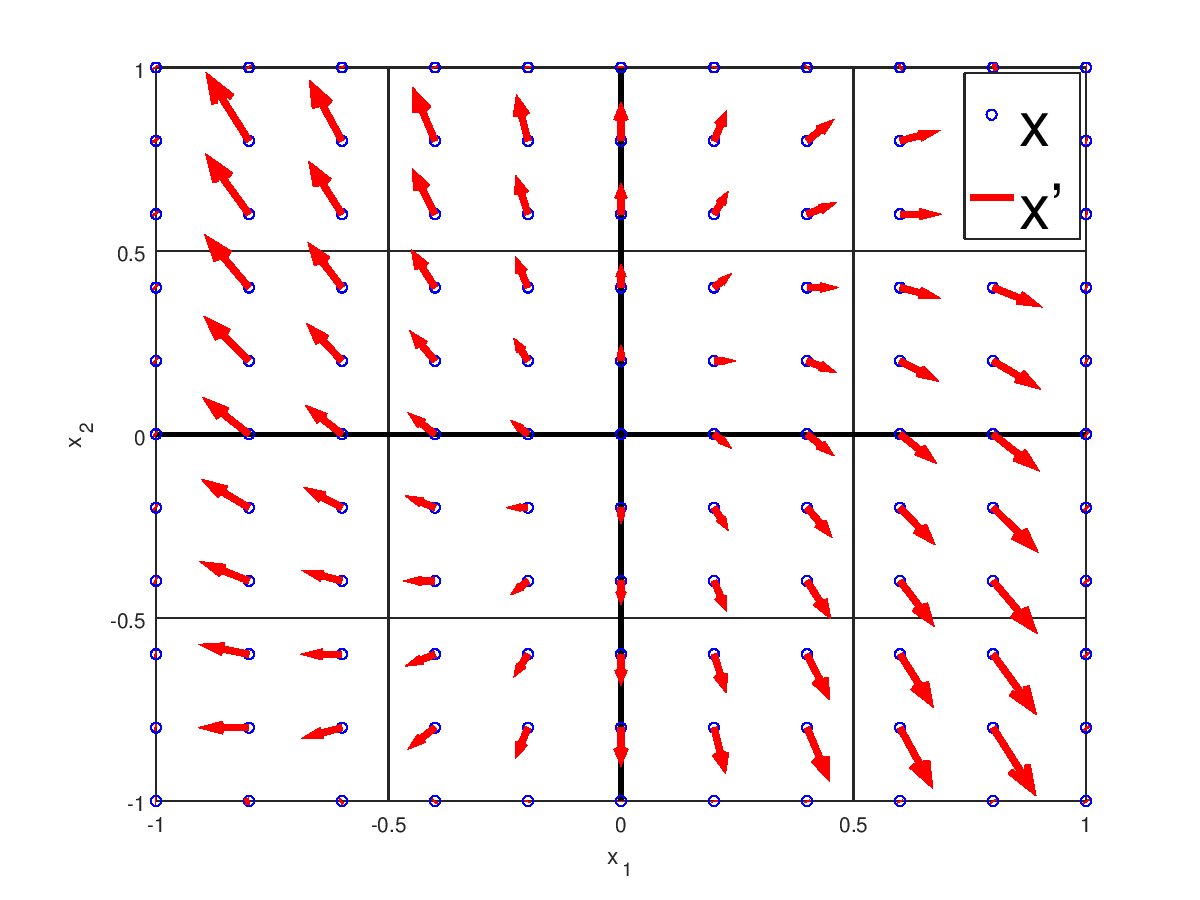
\includegraphics[width=0.25\textwidth]{A/20.png}
\end{document}
